\documentclass[conference]{IEEEtran}
\IEEEoverridecommandlockouts
% The preceding line is only needed to identify funding in the first footnote. If that is unneeded, please comment it out.
%Template version as of 6/27/2024

\usepackage{cite}
\usepackage{amsmath,amssymb,amsfonts}
\usepackage{algorithmic}
\usepackage{graphicx}
\usepackage{textcomp}
\usepackage{xcolor}
\usepackage{footmisc}
\usepackage{url}
\def\BibTeX{{\rm B\kern-.05em{\sc i\kern-.025em b}\kern-.08em
    T\kern-.1667em\lower.7ex\hbox{E}\kern-.125emX}}
\begin{document}

\title{Deep Reinforcement Learning for Traffic Light Control}

\author{\IEEEauthorblockN{Ben Bekir Ertugrul}
\IEEEauthorblockA{\textit{School of Engineering} \\
\textit{Jönköping University}\\
Jönköping, Sweden}
}

\maketitle

\begin{abstract}
This document is a model and instructions for \LaTeX.
This and the IEEEtran.cls file define the components of your paper [title, text, heads, etc.]. *CRITICAL: Do Not Use Symbols, Special Characters, Footnotes, 
or Math in Paper Title or Abstract.
\end{abstract}

\begin{IEEEkeywords}
component, formatting, style, styling, insert.
\end{IEEEkeywords}

\section{Introduction}
- What are SUMO limitations?
- Do we optimize traffic lights only for cars or also bikes, pedestrians, etc.
- Do we focus on multiple intersections or just one?
- Are we using acyclical or cyclical light switches? May one of them be more realistic than the other? 
- Do we train on multiple scenarios, like “rush hours” and low traffic conditions, or do we only have normal traffic?
- Do we use DQN or are there also other choices like PPO (is PPO able to combine with neural nets?)?

a good starting tutorial on how to generate traffic scenarios can be found here \cite{sumotutorial}.

- at the end, compare normal (static) traffic light with our solution. if possible, the static traffic light control should be decently good. maybe its possible to use a real example?

\section{Networks}

\subsection{Jönköping}
map of sweden downloaded here: https://download.geofabrik.de/europe/sweden.html
geojson polygon object created here: https://geojson.io/
chosen geojson found here\footnote{\url{https://github.com/benbekir/traffic-rl/blob/main/simulations/networks/jkpg/artifacts/jkpg.geojson}}.

\begin{figure}[h]
\label{fig:geojson-filter}
\centering
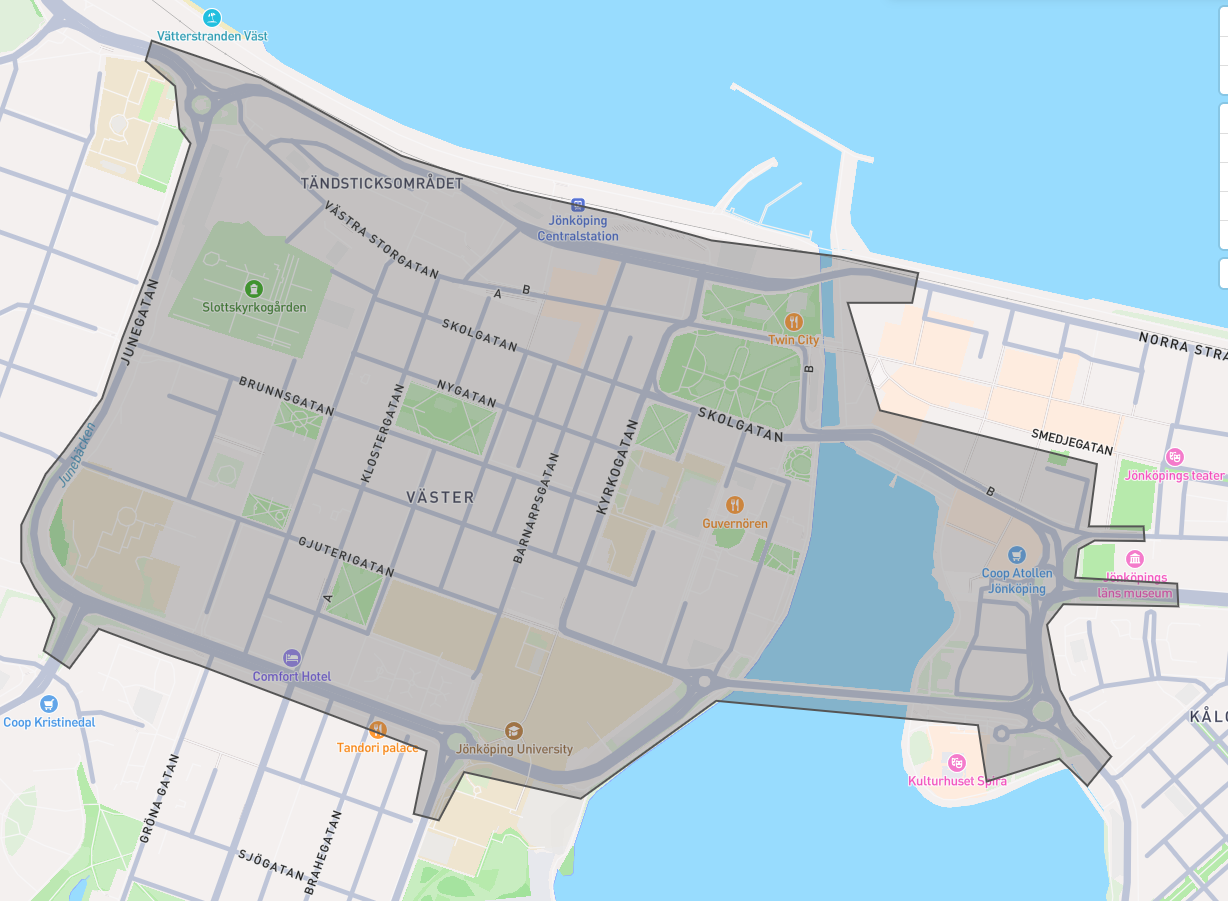
\includegraphics[width=\columnwidth]{resources/geojson_filter.png}
\caption{The filter (in grey) that defines the boundaries of the road network in Jönköping.}
\end{figure}

then, we used osmium and osmfilter to apply the polygon shape to the map of sweden. afterwards, we filter only for highways, except for those of the following types:

\begin{itemize}
    \item footway
    \item path
    \item pedestrian
    \item steps
    \item cycleway
    \item bridleway
\end{itemize}

finally, we use the SUMO \textit{netconvert} tool to convert the map into a SUMO network.

as for limitations, we extract lanes, intersections, and traffic lights, but do not have information about the speed limits on the roads. therefore, our simulation will treat every road the same.

\begin{figure}[h]
\label{fig:net}
\centering
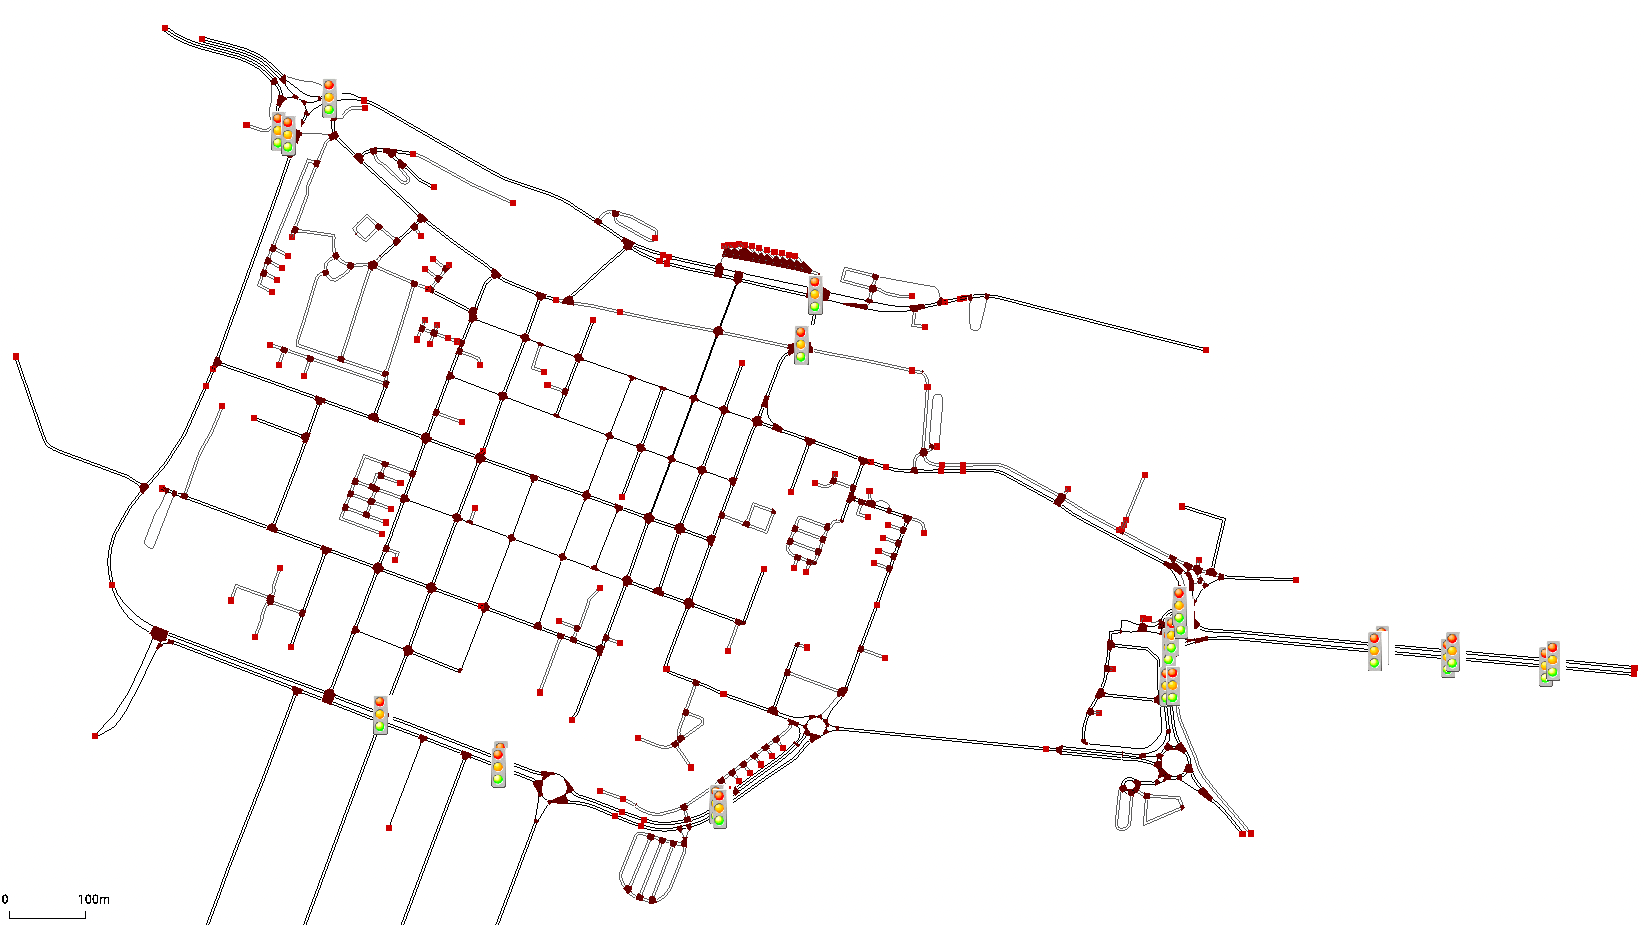
\includegraphics[width=\columnwidth]{resources/net.png}
\caption{The network as shown in the SUMO nededit UI, highlighting the traffic light placements.}
\end{figure}

\subsubsection{Demand Modeling}
since there is no publicly available data regarding traffic assignment zones and demand in jönköping, we use the SUMO tool randomTrips \footnote{\url{https://sumo.dlr.de/docs/Tools/Trip.html#randomtripspy}} with the random seed set to 12 to randomly create trips. we create 3600 individual trips in total where a new trip is spawned into the simulation on every timestep.

\subsubsection{Rush Hours and Noise}
im not sure about this yet

\subsubsection{Detectors}
To retrieve information that our agents can use, there are a couple of detector options that we could add to our environment (see \url{https://sumo.dlr.de/docs/Simulation/Output/#simulated_detectors}).

\begin{itemize}
    \item Inductive loop detectors
    \item Instant induction loops
    \item Lane area detectors
    \item Multi-Entry-Exit detectors
    \item Route detectors
\end{itemize}

we decide to use lane area detectors since they simulate vehicle tracking cameras, which gain popularity in the real world (i think in china especially) and provide rich information.  
these detectors are placed on every lane at every intersection that has a traffic light. the maximum length of the recorded lane segment is 25 meter.

\bibliographystyle{IEEEtran}
\bibliography{abrv,references}
\end{document}